\section[Podstawy teoretyczne (Piotr Winkler)]{Podstawy teoretyczne}

  W dzisiejszych czasach sieci neuronowe zajmują ważną pozycję na rynku narzędzi
  do edycji obrazu. Jest to głównie spowodowane ich umiejętnością do
  reprodukowania i modelowania nieliniowych procesów, a także nowoczesnymi
  technikami przetwarzania plików graficznych.
  Jednak pierwsze architektury ANN (ang. artificial neural network) nie nadawały
  się do przetwarzania grafik.
  Było to częściowo spowodowane faktem, że obrazy, będące w rzeczywistości macierzami
  wartości pikseli,
  % należało przekształcić w długie wektory liczbowe aby móc podać je
  ciężko było skutecznie podać
  na wejście typowych architektur DNN (ang. deep neural network) zbudowanych
  pierwotnie z wielu warstw ukrytych, pomiędzy którymi połączenia są na zasadzie
  każdy z każdym oraz posiadają swoje wagi podlegające modyfikacji w trakcie procesu
  uczenia. Taka struktura pokazana została na Rysunku \ref{fig:dnn}.
  Obrazy o niskiej rozdzielczości można było przekształcić w wektory
  wartości poszczególnych pikseli i w takiej postaci podawać na wejście sieci,
  jednak w przypadku obrazów o wyższej rozdzielczości to rozwiązanie, ze
  względu na znaczną długość powstałych wektorów, nie oferowało dobrych
  rezultatów.
  Dopiero nowe architektury sieci spowodowały przełom w tej dziedzinie.
  Wprowadzenie do najistotniejszych i najciekawszych z nich zostanie przedstawione w
  poniższym rozdziale, a także rozwinięte w dalszej części tej pracy.


  \begin{figure}[h]
    \centering
    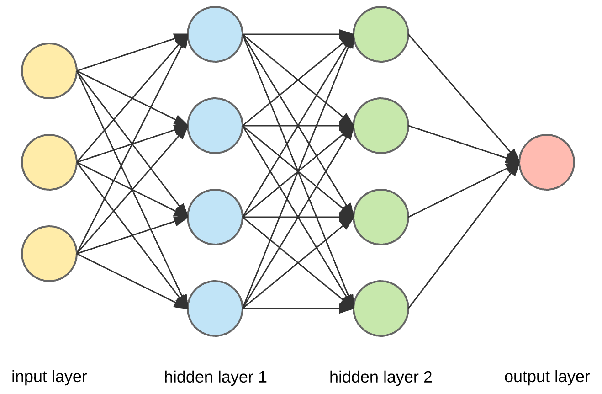
\includegraphics[width=4in]{dnn}
    \caption[Struktura DNN - źródło: \url{https://towardsdatascience.com/building-a-convolutional-neural-network-male-vs-female-50347e2fa88b}]{Struktura DNN}
    \label{fig:dnn}
  \end{figure}

  % Jedną z takich przełomowych architektur jest CNN (ang. convolutional neural
  % network). Są to sieci o hierarchicznej strukturze, gdzie obrazy wejściowe w
  % postaci macierzy wpier poddawane są ekstrakcji cech poprzez dokonanie operacji
  % konwolucji na obrazie poprzez przesuwanie zestawu filtrów wzdłuż obrazu.
  % Filtry te są zazywczaj inicjowane losowymi wartościami i w miarę trenowania,
  % dopasowują swoje parametry do wybranej problematyki.
  % Na wyjściu filtrów otrzymuje się macierze o mniejszej rozdzielczości
  % reprezentujące wyniki operacji konwolucji w danym punkcie. Otrzymane macierze
  % wyjściowe mogą być podawane na kolejne warstwy konwolucyjne w celu ekstrakcji
  % kolejnych cech. Dzięki temu procesowi kolejne warstwy filtrów uczą się
  % rozpoznawać kluczowe cechy na obrazie, od drobnych elemtów takich jak
  % krawędzie albo kształty po bardziej złożone takie jak części ciała albo
  % przedmioty.
  % Końcowe warstwy dokonują spłaszczania, czyli zamieniania wielowymiarowych
  % macierzy cech na jednowymiarowe wektore, które podawane są na wejście
  % FCL (ang. fully connected layer).

  % Lata rozwoju sztucznych sieci neuronowych zaowocowały powstaniem wielu technik służących do analizy i edycji obrazów. W poniższym rozdziale zaprezentowane zostaną, oraz pokrótce opisane, najważniejsze i najciekawsze przykłady, z których część znajdzie rozwinięcie w dalszej części tej pracy.

  \subsection{Sieci splotowe}
    \label{sieci_splotowe}

    Neuronowe sieci splotowe CNN (ang. convolutional neural network) stanowią podstawową strukturę w zakresie przetwarzania i analizowania obrazów cyfrowych. Są to sieci o hierarchicznej strukturze stanowiące podwaliny większości klasyfikatorów, detektorów, czy sieci segmentujących.

    Autorzy jednego z artykułów traktujących o sieciach splotowych \cite{cnn} opisują je następująco:
    \begin{quote}
      'CNN to skuteczny algorytm poznawczy, stosowany powszechnie przy rozpoznawaniu wzorców i przetwarzaniu obrazów. Posiada wiele cech, takich jak prosta struktura, mniej parametrów treningowych, czy zdolność do adaptacji. CNN stały się gorącym tematem w zakresie analizy głosu i rozpoznawania obrazu. Ich struktura oparta na podziale wag czyni je bardziej podobnymi do biologicznych sieci neuronowych. Redukuje to złożoność modelu sieci oraz liczbę wag'.
    \end{quote}

    \noindent
    Na CNN składają się zazwyczaj trzy rodzaje warstw, z których każda posiada inne cechy.

    Podstawową warstwę stanowi warstwa splotowa. Składa się ona ze zbioru filtrów (neuronów) odpowiedzialnych za ekstrakcję cech z analizowanych obrazów poprzez dokonanie operacji
    konwolucji na obrazie polegającej na przesuwaniu zestawu filtrów wzdłuż niego.
    Na wyjściu filtrów otrzymuje się macierze o mniejszej rozdzielczości
    reprezentujące wyniki operacji konwolucji w danym punkcie. Każda kolejna warstwa splotowa wydobywa z obrazu cechy o wyższych poziomach abstrakcji
    bazując na wynikach obliczeń poprzednich warstw tego rodzaju. Dzięki temu
    procesowi kolejne warstwy filtrów uczą się
    rozpoznawać kluczowe cechy na obrazie, od drobnych elementów takich jak
    krawędzie albo kształty po bardziej złożone takie jak części ciała albo
    całe obiekty. Filtry te są zazwyczaj inicjowane losowymi wartościami i w miarę trenowania, dopasowują swoje parametry do wybranej problematyki.

    Drugim istotnym elementem sieci splotowych jest warstwa poolingu. Może zostać opisana następująco \cite{deeplearn}:
    \begin{quote}
      'We wszystkich przypadkach pooling pomaga uczynić reprezentację w przybliżeniu niezmienną w stosunku do małych tłumaczeń danych wejściowych. Niezmienność wobec tłumaczenia oznacza, że jeśli poddamy dane wejściowe nieznacznej translacji, to wartość większości wyników poddanych poolingowi nie ulegnie zmianie'.
    \end{quote}

    Końcowy element CNN w większości przypadków stanowią warstwy gęste (FCL ang. Fully Connected Layer). Odpowiadają one za dokonanie odpowiedniej klasyfikacji obrazu na podstawie danych dostarczonych przez warstwy poprzedzające. Są przez to nieodzowne w przypadku zadań związanych z wszelkiego rodzaju klasyfikacją obrazów.

    Wymienione tutaj elementy składowe sieci splotowych mogą przyjmować różne rozmiary i występować w różnych konfiguracjach, co przedstawiono na poniższym Rysunku \ref{fig:cnn_structure}.
    \begin{figure}[h]
     \centering
     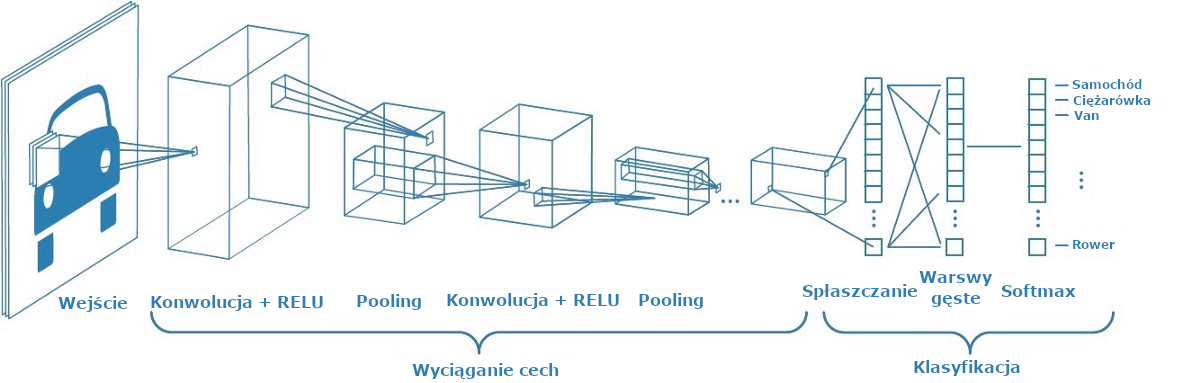
\includegraphics[width=4in]{cnn_structure}
     \caption[Przykładowa struktura CNN - źródło: \url{https://www.mathworks.com/solutions/deep-learning/convolutional-neural-network.html}]{Przykładowa struktura CNN}
     \label{fig:cnn_structure}
    \end{figure}
    \newline
    Zapewnia to szerokie pole do eksperymentów i sprawia, że sieci te zdolne są rozwiązywać złożone, różnorodne problemy z wielu dziedzin codziennego życia.

  \subsection{FCN}

   Jednym z kluczowych problemów, jakie stawia przed badaczami edycja obrazów jest zagadnienie segmentacji semantycznej. Klasyczna klasyfikacja, polegająca na przypisywaniu obrazów do odpowiednich grup tematycznych, jest w tym przypadku sprowadzana do poziomu pojedynczych pikseli. Oznacza to, że sieci neuronowe przeznaczone do tego zadania są w stanie dokonać klasyfikacji dla każdego pojedynczego piksela analizowanego obrazu. Na tej podstawie uzyskiwany jest podział na segmenty, z których każdy reprezentuje inną klasę obiektów, jak na poniższym Rysunku \ref{fig:segmentation}.

   \begin{figure}[h]
    \centering
    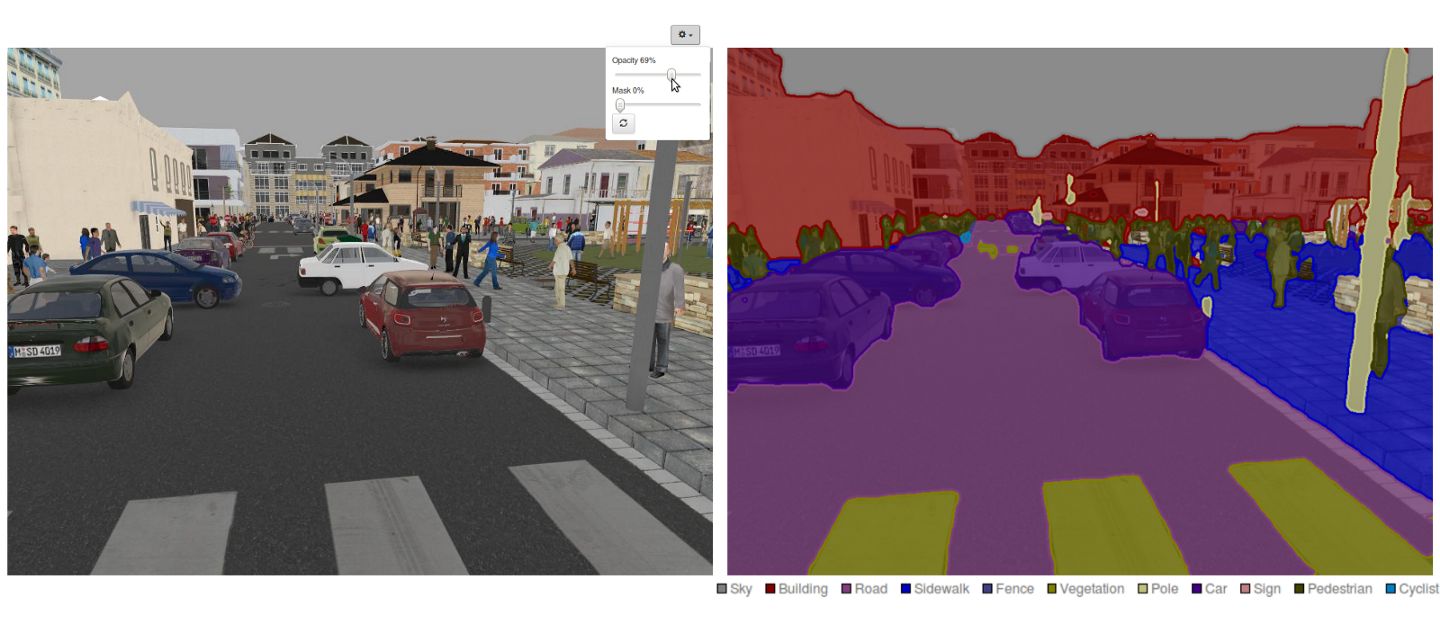
\includegraphics[width=4in]{segmentation}
    \caption[Segmentacja semantyczna - źródło: \url{https://devblogs.nvidia.com/image-segmentation-using-digits-5/}]{Segmentacja semantyczna}
    \label{fig:segmentation}
  \end{figure}

   W większości modele odpowiadające za przeprowadzanie segmentacji składają się z szeregowego połączenia enkodera oraz dekodera. Enkoder jest zazwyczaj pre-trenowaną siecią neuronową przeznaczoną do klasyfikowania obrazów. Dekoder odpowiada za semantyczne rzutowanie cech w niskiej rozdzielczości, wyuczonych przez enkoder, na wysoką rozdzielczość samych pikseli tworząc wspomniany wcześniej podział segmentowy.

   FCN (ang. Fully Convolutional Networks) stanowią szczególny rodzaj sieci neuronowych przeznaczonych do segmentacji obrazów. Składają się one wyłącznie z kombinacji warstw splotowych oraz poolingu. Są w stanie przetwarzać obrazy o dowolnej, zmiennej wielkości, w odróżnieniu od innych typów modeli, w których zastosowanie warstw gęstych (FCL) wymusza z góry ustalone rozmiary danych wejściowych.

   Naprzemienne przepuszczanie obrazów przez wspomniane warstwy splotowe oraz pooling może powodować niską rozdzielczość wyjściowych rezultatów pracy tych sieci oraz rozmycie granic poszczególnych obiektów. Z tego powodu w nowoczesnych rozwiązaniach stosuje się dodatkowe mechanizmy zapobiegające tego typu trendom.

  \subsection{Modele generatywne}
  \label{modele_generatywne}
   Koncepcja modeli generatywnych, w skrócie GANów, przedstawiona została w 2014 roku przez Iana Goodfellow oraz jego współpracowników na uniwersytecie w Montrealu \cite{gan}. Modele te stanowią połączenie dwóch głębokich sieci neuronowych działających przeciwstawnie do siebie nawzajem.

   Pierwsza sieć to tak zwany generator. W odniesieniu do tematu pracy, jego działanie polega na generowaniu nowych obrazów, lub ich fragmentów na podstawie wektora szumów.

   Obrazy te przekazywane są, równolegle z zestawem obrazów prawdziwych, do dyskryminatora stanowiącego drugą część modelu GAN. Działanie tej sieci neuronowej polega na określeniu (w skali 0 do 1), w jakim stopniu produkty wyjściowe generatora odpowiadają obrazom rzeczywistym.

   W opisanym modelu występuje zatem podwójna pętla sprzężenia zwrotnego. Dyskryminator określa autentyczność obrazów porównując je ze zdefiniowaną odgórnie bazą danych. Z kolei generator otrzymuje informację o skuteczności swojego działania ze strony dyskryminatora.

   Model generatywny znajduje się w stanie ciągłego konfliktu. Generator dąży do jak najdokładniejszego fałszowania obrazów w celu oszukania dyskryminatora, którego celem jest z kolei jak najdokładniejsze wykrywanie podróbek. Obie sieci neuronowe nieustannie dążą do osiągnięcia przewagi nad rywalem w procesie treningu. Ciągła rywalizacja sprawia, że zarówno generator, jak i dyskryminator zyskują coraz wyższą skuteczność działania.

   W praktyce modele generatywne są w stanie naśladować dowolną dystrybucję danych. Są w stanie kreować światy podobne do naszego w zakresie obrazu, dźwięku czy mowy. Można powiedzieć, że są to prawdziwi syntetyczni artyści.
